%%%%%%%%%%%%%%%%%%%%%%%%%%%%%%%%%%%%%%%%%%%%%%%%
% Template TCMN data sheet version 3
% 
% Alberto Sanchez asanchezrodelgo@ifc.org Dec 2015
%%%%%%%%%%%%%%%%%%%%%%%%%%%%%%%%%%%%%%%%%%%%%%%%
\documentclass{article}\usepackage[]{graphicx}\usepackage[]{color}
%% maxwidth is the original width if it is less than linewidth
%% otherwise use linewidth (to make sure the graphics do not exceed the margin)
\makeatletter
\def\maxwidth{ %
  \ifdim\Gin@nat@width>\linewidth
    \linewidth
  \else
    \Gin@nat@width
  \fi
}
\makeatother

\definecolor{fgcolor}{rgb}{0.345, 0.345, 0.345}
\newcommand{\hlnum}[1]{\textcolor[rgb]{0.686,0.059,0.569}{#1}}%
\newcommand{\hlstr}[1]{\textcolor[rgb]{0.192,0.494,0.8}{#1}}%
\newcommand{\hlcom}[1]{\textcolor[rgb]{0.678,0.584,0.686}{\textit{#1}}}%
\newcommand{\hlopt}[1]{\textcolor[rgb]{0,0,0}{#1}}%
\newcommand{\hlstd}[1]{\textcolor[rgb]{0.345,0.345,0.345}{#1}}%
\newcommand{\hlkwa}[1]{\textcolor[rgb]{0.161,0.373,0.58}{\textbf{#1}}}%
\newcommand{\hlkwb}[1]{\textcolor[rgb]{0.69,0.353,0.396}{#1}}%
\newcommand{\hlkwc}[1]{\textcolor[rgb]{0.333,0.667,0.333}{#1}}%
\newcommand{\hlkwd}[1]{\textcolor[rgb]{0.737,0.353,0.396}{\textbf{#1}}}%

\usepackage{framed}
\makeatletter
\newenvironment{kframe}{%
 \def\at@end@of@kframe{}%
 \ifinner\ifhmode%
  \def\at@end@of@kframe{\end{minipage}}%
  \begin{minipage}{\columnwidth}%
 \fi\fi%
 \def\FrameCommand##1{\hskip\@totalleftmargin \hskip-\fboxsep
 \colorbox{shadecolor}{##1}\hskip-\fboxsep
     % There is no \\@totalrightmargin, so:
     \hskip-\linewidth \hskip-\@totalleftmargin \hskip\columnwidth}%
 \MakeFramed {\advance\hsize-\width
   \@totalleftmargin\z@ \linewidth\hsize
   \@setminipage}}%
 {\par\unskip\endMakeFramed%
 \at@end@of@kframe}
\makeatother

\definecolor{shadecolor}{rgb}{.97, .97, .97}
\definecolor{messagecolor}{rgb}{0, 0, 0}
\definecolor{warningcolor}{rgb}{1, 0, 1}
\definecolor{errorcolor}{rgb}{1, 0, 0}
\newenvironment{knitrout}{}{} % an empty environment to be redefined in TeX

\usepackage{alltt}
%%%%%%%%%%%%%% package declaration %%%%%%%%%%%%%%%%%%%%%
\usepackage[top=0.3in, bottom=0.1in, left=0.5in, right=0.6in]{geometry}
\usepackage{graphicx} % to load images
\usepackage[export]{adjustbox} % add alignment to includegraphics
\usepackage[font=small]{caption}
\usepackage{xcolor} % color text
\usepackage{tabularx} % to adjust table width, etc. 
\usepackage{titlesec} % format titles and headers
\usepackage{sectsty} % format sections & subsections
\usepackage{booktabs} % For \toprule, \midrule and \bottomrule
\usepackage[colorlinks = true,
            linkcolor = blue,
            urlcolor  = blue,
            citecolor = blue,
            anchorcolor = blue]{hyperref} % to include hyperlinks in the doc
\sectionfont{\fontsize{16}{15}\selectfont\raggedright} % formats title newsletter (section) 
\subsectionfont{\fontsize{14}{12}\selectfont\raggedright} % formats title newsletter (section)
%%%%%%%%%%%%%%%%%%%%%%%%%%%%%%%%%%%%%%%%%%%%%%%%%%%%%%%%%%%%%%%%%%%%%%%%%%%%%%%%%%%
%
%%%%%%%%%%%%%%%%%%%%%%%%%%%%%%%%%%%%% BEGIN DOCUMENT %%%%%%%%%%%%%%%%%%%%%%%%%%%%%%
\IfFileExists{upquote.sty}{\usepackage{upquote}}{}
\begin{document}

%

%%%%%%%%%%%%%%%% PAGE 1 %%%%%%%%%%%%%%%%%%%
%World Bank logo and TCMN branding
\begin{figure}
  \vspace{-3ex} % move up this figure
  \hspace{-7ex} % move left this figure
  \includegraphics[width=5cm]{/Users/asanchez3/shinyTCMN/www/wb_logo_background.png}
\end{figure}
\begin{figure}
  \begin{minipage}[t]{0.99\textwidth} % top section
      \vspace{-30ex}
      \hspace{-2ex}
      \raggedright{\includegraphics[width=5.5cm,right]{/Users/asanchez3/shinyTCMN/www/TC_snapshots_data.png}}
  %  {\color{white!70!black}\noindent\makebox[\linewidth]{\rule{20cm}{0.3pt}}} % horiz line
  \end{minipage}
\end{figure}
%
%%%% Macro Indicators
\begin{minipage}[t]{0.99\textwidth} % top section
  \vspace{-1.5cm}
  \begin{minipage}[c]{0.36\textwidth} 
    \begin{minipage}[c]{0.28\textwidth} % flag
      \includegraphics[width=1.2cm,height=1.2cm]{/Users/asanchez3/shinyTCMN/www/BD.png}
    \end{minipage}
    \begin{minipage}[c]{0.70\textwidth} % Country name
      \section*{\color{blue!40!black}Bangladesh}
    \end{minipage}
  \end{minipage}
  \begin{minipage}[c]{0.63\textwidth} % key macro table 
    % Table 1
    \centering
    \resizebox{\textwidth}{!}{
% latex table generated in R 3.2.2 by xtable 1.7-4 package
% Tue May 31 11:05:31 2016
{\LARGE
\begin{tabular}{>{\centering}p{1.5in}>{\centering}p{1.5in}>{\centering}p{1.5in}>{\centering}p{1.5in}>{\centering}p{1.5in}>{\centering}p{1.5in}>{\centering}p{1.5in}l}
  GDP (US\$ billions) (2017) & Population (millions) (2017) & Land area (sq. km) (2015) & Income per capita (current US\$) (2017) & Poverty rate (2010) \large{[1]} & Unemployment rate (2016) & Ease of Doing Business Rank (2016) &  \\ 
      257 &     165 & 130,170 &   1,556 &      44 &      NA &     174 &  \\ 
  \end{tabular}
}

    }
  \end{minipage}  
\end{minipage} % end top section

\begin{minipage}[b]{0.99\textwidth} % macro indicators main table
  %\vspace*{0.5cm}
  %\vspace{+3ex}
  \begin{minipage}[t]{0.99\textwidth}

    \begin{minipage}[c]{0.875\textwidth}
      \begin{flushleft}  
      {\color{white!30!blue} \textbf{\small Macro Indicators}}
      \end{flushleft} 
      \vspace*{-0.4cm}
      % Table 2
      \centering
      \resizebox{\textwidth}{!}{
% latex table generated in R 3.2.2 by xtable 1.7-4 package
% Tue May 31 11:05:31 2016
{\Large
\begin{tabular}{>{\raggedright}p{6in}r>{\raggedleft}p{0.8in}>{\raggedleft}p{0.8in}>{\raggedleft}p{0.8in}>{\raggedleft}p{0.8in}>{\raggedleft}p{0.8in}l}
  & Avg 2003-2012 & 2013 & 2014 & 2015 & 2016 & 2017 &  \\ 
  \hline
GDP growth (annual \%) &   5.73 &   6.03 &   6.06 &   6.51 &   6.50 &   6.70 &  \\ 
  Current account balance &   0.57 &   1.59 &   0.81 &  -0.85 &  -0.40 &  -0.60 &  \\ 
  Fiscal balance (\% of GDP) &  -3.46 &  -3.87 &  -3.48 &  -3.58 &  -4.57 &  -4.44 &  \\ 
  Remittances, received (\% of GDP) \large{[1]} &   8.27 &   9.25 &   8.67 & --- & --- & --- &  \\ 
  General government gross debt \large{[3]} &  40.02 &  34.47 &  33.87 &  33.95 &  34.32 & --- &  \\ 
  Real Effective Exchange Rate (2010=100) &  94.53 & 103.36 & 114.06 & 131.70 & 136.36 & 142.80 &  \\ 
  Consumer Price Index, annual percent change &   7.33 &   6.81 &   7.31 &   6.45 &   6.47 &   6.71 &  \\ 
  \end{tabular}
}

      }
    \end{minipage}
    \begin{minipage}[c]{0.11\textwidth}
      \vspace*{+0.8cm}


{\centering 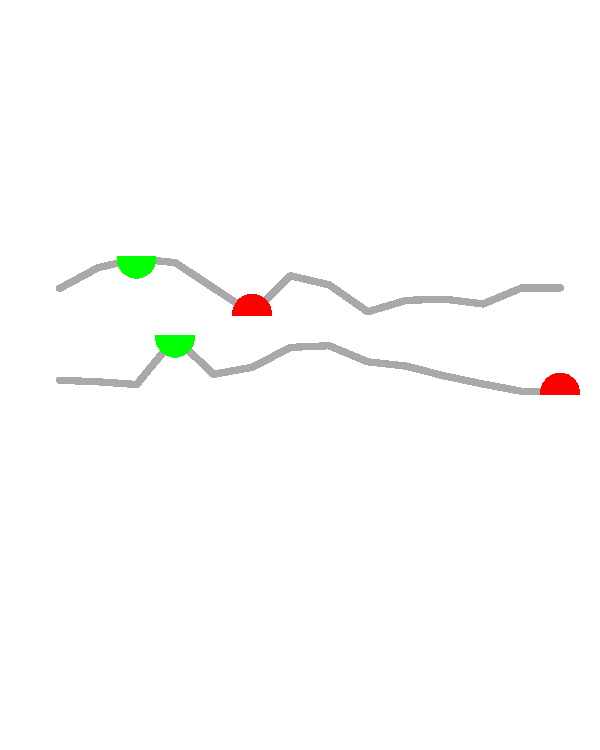
\includegraphics[width=\maxwidth]{figure/createSparklines_macro-1} 

}



      \vspace*{-0.5cm}
    \end{minipage}
    
    %\vspace*{-0.4cm}
    \begin{minipage}[c]{0.875\textwidth}
      \begin{flushleft}  
      {\color{white!30!blue} \textbf{\small Investment indicators}}
      \end{flushleft} 
      \vspace*{-0.4cm}
      % Table 2
      \centering
      \resizebox{\textwidth}{!}{
% latex table generated in R 3.2.2 by xtable 1.7-4 package
% Tue May 31 11:05:31 2016
{\Large
\begin{tabular}{>{\raggedright}p{6in}r>{\raggedleft}p{0.8in}>{\raggedleft}p{0.8in}>{\raggedleft}p{0.8in}>{\raggedleft}p{0.8in}>{\raggedleft}p{0.8in}l}
  & Avg 2003-2012 & 2013 & 2014 & 2015 & 2016 & 2017 &  \\ 
  \hline
Gross domestic investment (\% GDP) & 25.93 & 30.25 & 31.33 & 32.23 & 32.51 & 32.79 &  \\ 
  Gross domestic investment, of w: Private investment (\% GDP) \large{[1]} & 26.22 & 28.39 & 28.58 & --- & --- & --- &  \\ 
  Inward FDI (\% of GDP) \large{[2]} &  0.89 &  1.04 &  0.87 & --- & --- & --- &  \\ 
  Inward FDI, \% of private investment \large{[2]} &  3.37 &  3.67 &    NA & --- & --- & --- &  \\ 
  \end{tabular}
}

      }
    \end{minipage}
    \begin{minipage}[c]{0.11\textwidth}
      \vspace*{+0.8cm}


{\centering 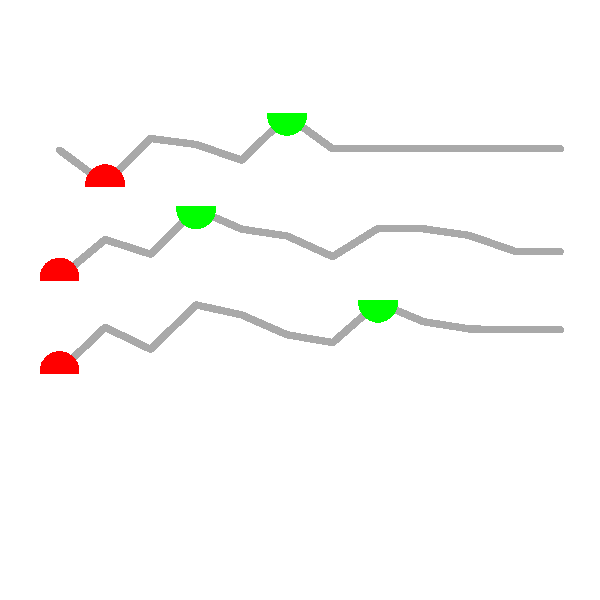
\includegraphics[width=\maxwidth]{figure/createSparklines_invest-1} 

}



      \vspace*{-0.5cm}
    \end{minipage}
    
    %\vspace*{-0.4cm}
    \begin{minipage}[c]{0.875\textwidth}
      \begin{flushleft}  
      {\color{white!30!blue} \textbf{\small Trade Indicators}}
      \end{flushleft} 
      \vspace*{-0.4cm}
      % Table 2
      \centering
      \resizebox{\textwidth}{!}{
% latex table generated in R 3.2.2 by xtable 1.7-4 package
% Tue May 31 11:05:31 2016
{\Large
\begin{tabular}{>{\raggedright}p{6in}r>{\raggedleft}p{0.8in}>{\raggedleft}p{0.8in}>{\raggedleft}p{0.8in}>{\raggedleft}p{0.8in}>{\raggedleft}p{0.8in}l}
  & Avg 2003-2012 & 2013 & 2014 & 2015 & 2016 & 2017 &  \\ 
  \hline
Total Trade in Goods and Services (\% of GDP, real terms) & 30.4 & 42.9 & 41.3 & 39.6 & 41.1 & 42.8 &  \\ 
  Trade balance (\% GDP, real terms) & -4.0 & -3.5 & -3.0 & -5.0 & -5.8 & -6.3 &  \\ 
  Exports, Goods and Services, annual percent change (real terms) & 19.2 &  2.4 &  3.2 & -3.7 &  8.5 & 10.5 &  \\ 
  Imports, Goods and Services, annual percent change (real terms) & 17.4 &  1.2 &  1.2 &  7.5 & 12.0 & 11.5 &  \\ 
  Total reserves in months of imports \large{[1]} &  3.2 &  4.9 &  5.3 & --- & --- & --- &  \\ 
  \end{tabular}
}

      }
    \end{minipage}
    \begin{minipage}[c]{0.11\textwidth}
      \vspace*{+0.8cm}


{\centering 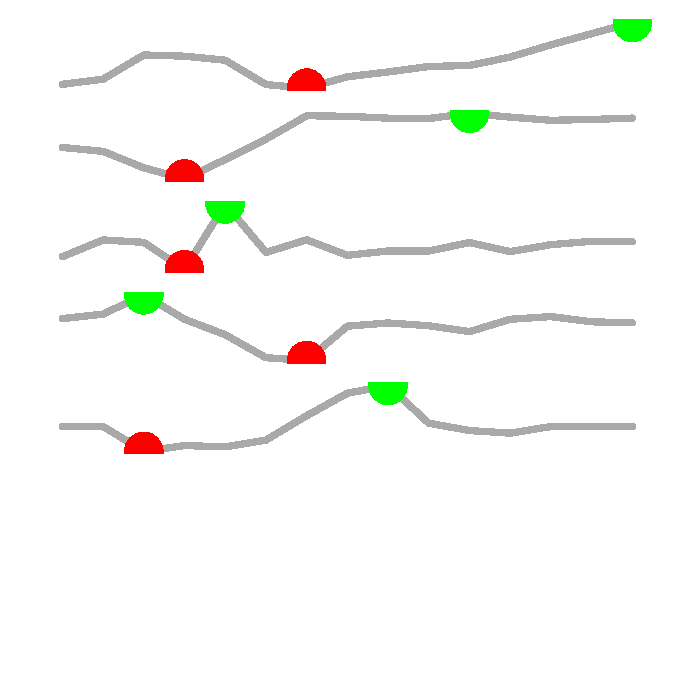
\includegraphics[width=\maxwidth]{figure/createSparklines_trade-1} 

}



      \vspace*{-0.4cm}
    \end{minipage}
  \\[3pt]
\raggedright{\footnotesize{\href{http://www.worldbank.org/en/topic/macroeconomics/overview}{Sources: MFM note}{,} \href{http://data.worldbank.org/data-catalog/world-development indicators}{[1] World Development Indicators (WDI)}{,} \href{http://unctadstat.unctad.org/wds/ReportFolders/reportFolders.aspx}{[2] UNCTADSTAT}{,} \href{https://www.imf.org/external/pubs/ft/weo/2015/02/weodata/index.aspx}{[3] World Economic Outlook (WEO)}}}
  \end{minipage} 
%\end{minipage}    
  \begin{minipage}[b]{\textwidth} % macro charts
  \vspace{+3ex}
    \begin{minipage}[c]{0.49\textwidth} % imports/exports 
    \center{\color{blue!50!black} \textbf{\small Goods Export and Import \\ volume growth, 2012-2015}}


{\centering 
\includegraphics[width=\maxwidth]{figure/ExpImp_HF-1} 

}



    \vspace*{-0.3cm}
    %\hspace*{0.5cm} 
    \raggedright{\footnotesize{\href{http://web.worldbank.org/WBSITE/EXTERNAL/EXTDEC/EXTDECPROSPECTS/0,,menuPK:476941~pagePK:51084723~piPK:51084722~theSitePK:476883,00.html}{Source: Development Prospects Group (DECPG)}}}
    \end{minipage}
    \begin{minipage}[c]{0.49\textwidth} % gdp value added
    \center{\color{blue!50!black} \textbf{\small Gross Value Added by \\ Economic Activity 2013 \footnotesize(\% GDP)}}


{\centering 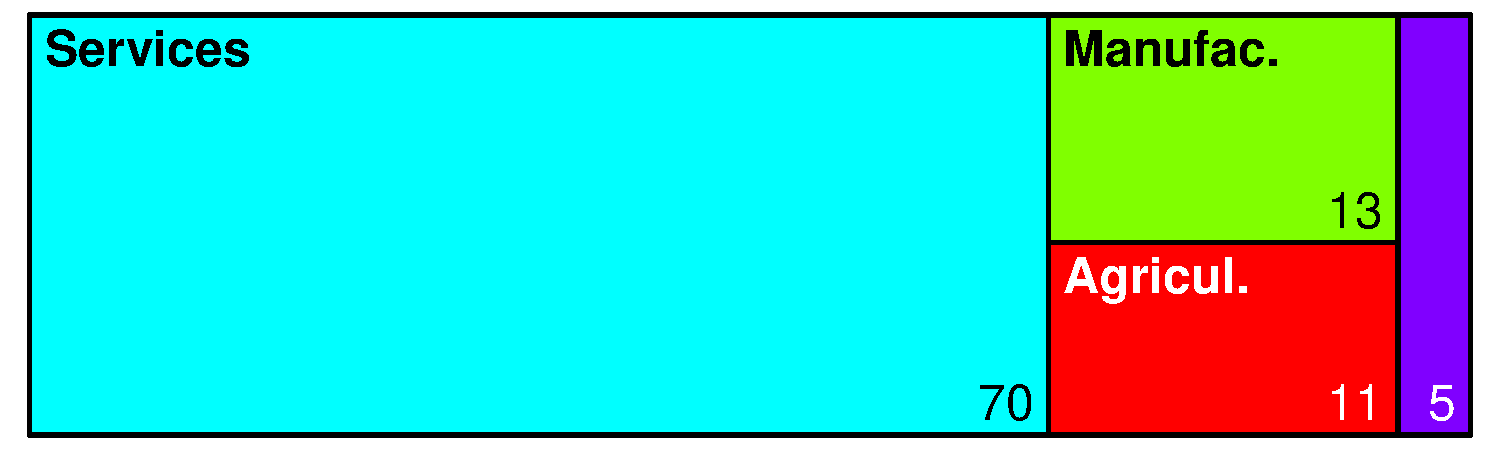
\includegraphics[width=\maxwidth]{figure/GVA_Treemap-1} 

}



   %\vspace*{-0.3cm}
   %\hspace*{0.5cm} 
   \raggedright{\footnotesize{\href{http://data.worldbank.org/data-catalog/world-development indicators}{Source: World Development Indicators (WDI)}}}
    \end{minipage}
  \end{minipage}  
\end{minipage}   
 
%%%% Exports Imports and DB
\begin{minipage}[b]{0.99\textwidth}
  \vspace{0.8cm}
   \begin{minipage}[c]{0.44\textwidth} 
    %\vspace*{-0.2cm}
    \begin{minipage}[t]{0.99\textwidth} 
      {\color{blue!50!black} \textbf{\small Top 5 Exports by \% of Total Value, 2011}}
      %\vspace{3ex}
      \\[6pt]
      \centering
      \resizebox{\textwidth}{!}{%


{\centering 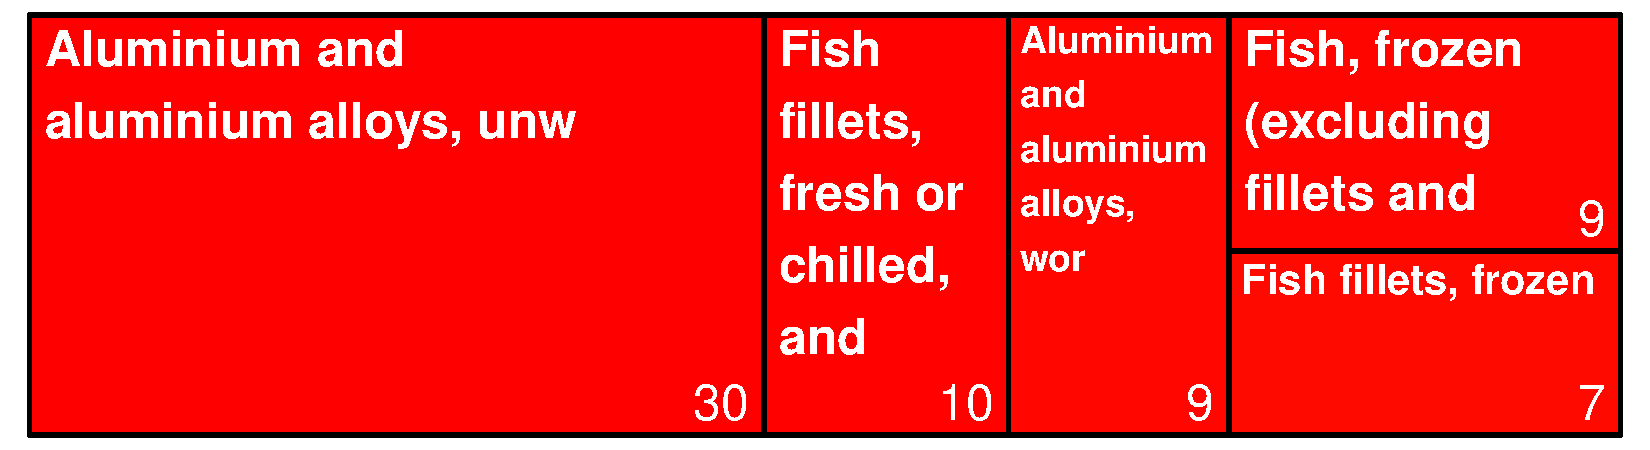
\includegraphics[width=\maxwidth]{figure/ImpExp_Treemap-2-1} 

}



      }
      \end{minipage}
      \\[14pt]
      \begin{minipage}[t]{0.99\textwidth} 
      {\color{blue!50!black} \textbf{\small Imports Categories by \% of Total Value, 2011}}
      \\[6pt]
      \centering
      \resizebox{\textwidth}{!}{%


{\centering 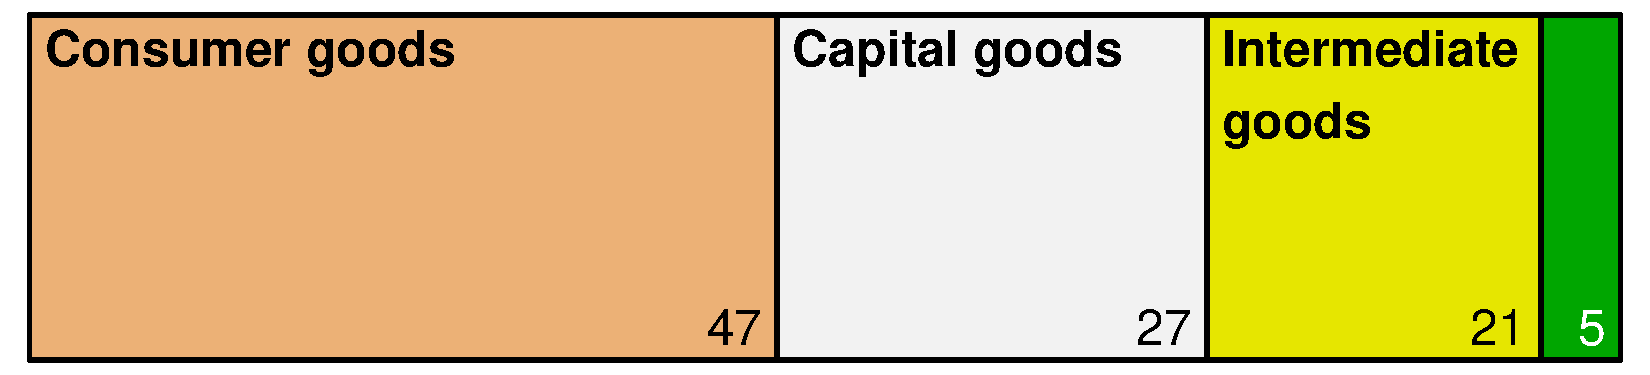
\includegraphics[width=\maxwidth]{figure/ImpExp_Treemap-1-1} 

}



      }
      \end{minipage}
      \\[10pt]
    %\hspace*{0.5cm}
    \footnotesize{\href{http://wits.worldbank.org}{Source: World Integrated Trade Solution (WITS)}} 
    \end{minipage}
    \begin{minipage}[c]{0.56\textwidth} % Doing Business table
    %\vspace*{-0.1cm}
    %\begin{flushleft}
      \center {\color{blue!50!black}\textbf{\small Doing Business 2015 \\ \footnotesize Distance to Frontier (DTF) and Rank}}
    %\end{flushleft}
    \\[18pt]
    \centering
      \resizebox{\textwidth}{!}{%
% latex table generated in R 3.2.2 by xtable 1.7-4 package
% Tue May 31 11:05:33 2016
{\large
\begin{tabular}{lrrr|rrrr}
  &  & DTF &  &  & Rank &  &  \\ 
  &  2015 &  2016 &  Change & 2015 & 2016 & Change &  \\ 
   \hline
\textbf{Ease of Doing Business} & \textbf{42.71} & \textbf{43.1} & \textbf{\color{green}{0.39}} & \textbf{172} & \textbf{174} & \textbf{\color{red}{-2}} &  \\ 
  Dealing with Construction Permits & 64.78 & 65.27 & \color{green}{0.49} & 118 & 118 & 0 &  \\ 
  Enforcing Contracts & 22.21 & 22.21 & 0 & 188 & 188 & 0 &  \\ 
  Getting Credit & 30 & 30 & 0 & 128 & 133 & \color{red}{-5} &  \\ 
  Getting Electricity & 12.99 & 15.31 & \color{green}{2.32} & 189 & 189 & 0 &  \\ 
  Paying Taxes & 73.98 & 74.42 & \color{green}{0.44} & 85 & 86 & \color{red}{-1} &  \\ 
  Protecting Minority Investors & 53.33 & 53.33 & 0 & 87 & 88 & \color{red}{-1} &  \\ 
  Registering Property & 27.26 & 27.48 & \color{green}{0.22} & 184 & 185 & \color{red}{-1} &  \\ 
  Resolving Insolvency & 26.36 & 26.36 & 0 & 155 & 155 & 0 &  \\ 
  Starting a Business & 81.36 & 81.72 & \color{green}{0.36} & 111 & 117 & \color{red}{-6} &  \\ 
  Trading Across Borders & 34.86 & 34.86 & 0 & 172 & 172 & 0 &  \\ 
  \end{tabular}
}

      }
    \\[15pt]
     %\hspace*{0.5cm} 
     \raggedright{\footnotesize{\href{http://www.doingbusiness.org/data}{Source: Doing Busines Report 2015}}}
    \end{minipage}
\end{minipage}

% \vspace{+3ex}
% {\color{blue!50!white}\noindent\makebox[\linewidth]{\rule{18cm}{0.3pt}}} % horiz line
% \begin{minipage}[c]{0.99\textwidth}
%   \hspace*{-0.4cm}\raggedleft{\color{white!40!black} \footnotesize TRADE AND COMPETITIVENESS MONITORING NOTE - UPDATED} 
%   %month year}
% \end{minipage}

\newpage
%%%%%%%%%%%%%%%% PAGE 2 %%%%%%%%%%%%%%%%%%%

\begin{minipage}[t]{0.99\textwidth}
  \vspace{0.5cm}
  \begin{minipage}[c]{0.48\textwidth} % WEF Radar
    \center{\color{blue!50!black} \textbf{WEF Competitiveness Indicators \\ \footnotesize(Scale 1-7, 7=best)}}
    \vspace*{-0.6cm}


{\centering 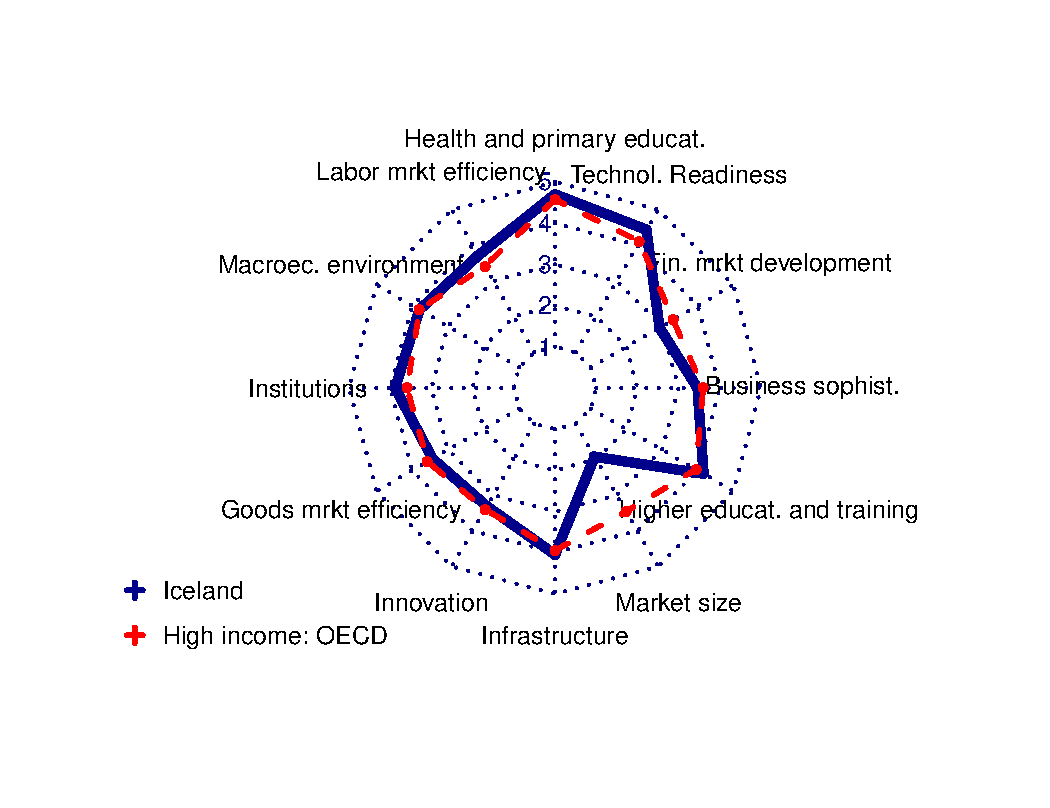
\includegraphics[width=\maxwidth]{figure/WEFradar-1} 

}



    \vspace*{-0.6cm} 
    \hspace*{0.3cm} \raggedright\footnotesize{\href{http://www.weforum.org/global-competitiveness-report-2015-2016}{Source: WEF Global Competitiveness Report 2015}}
  \end{minipage}
  \begin{minipage}[c]{0.50\textwidth} % LPI chart
  %\vspace*{0.5cm}
  \center {\color{blue!50!black} \textbf{Logistics Performance Index \\ \footnotesize(Scale 1-5, 5=best)}}
    \vspace*{0.4cm}


{\centering 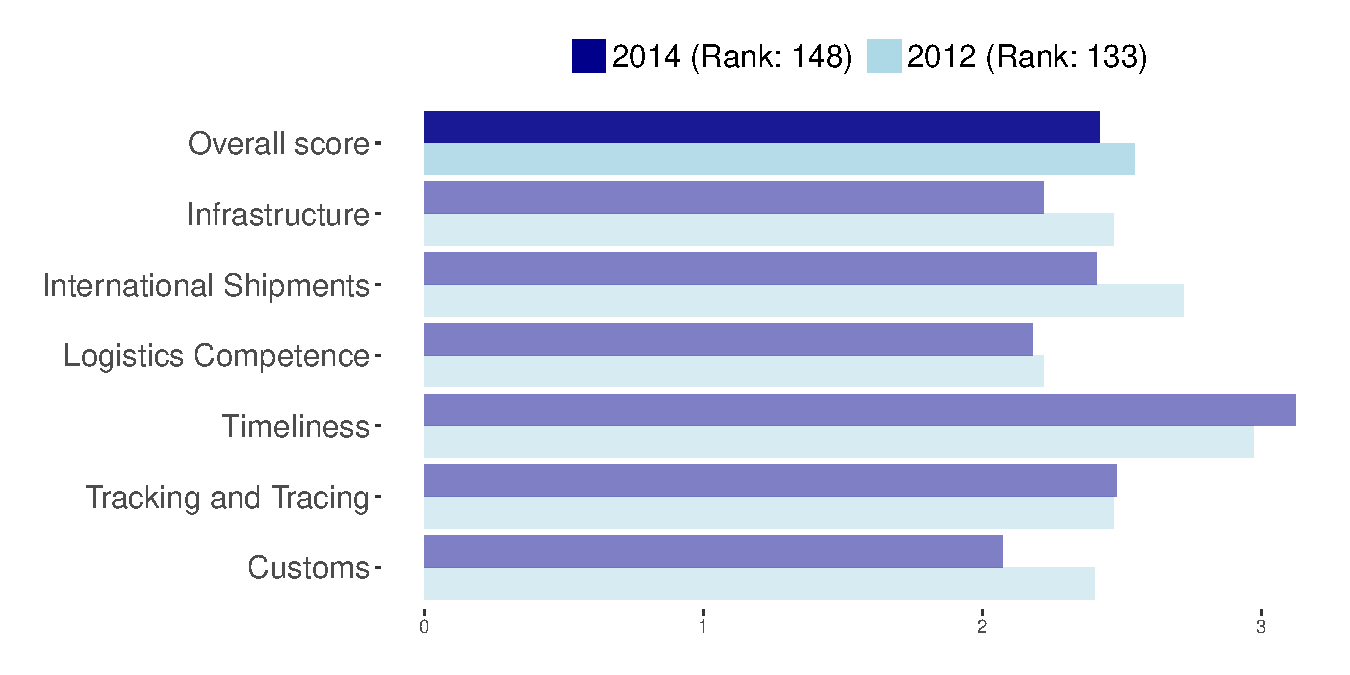
\includegraphics[width=\maxwidth]{figure/LPIindicators-1} 

}



  %\hspace*{0.5cm} 
  \raggedright\footnotesize{\href{http://lpi.worldbank.org}{Source: Logistics Performance Index (World Bank)}}
  \end{minipage}
\end{minipage}  

\begin{minipage}[b]{0.99\textwidth}
  \begin{minipage}[c]{0.50\textwidth} % WGI chart
    \vspace*{0.8cm}
    \center {\color{blue!50!black} \textbf{World Governance indicators \\ \footnotesize(Std. score, High=best)}}
    \vspace*{0.3cm}


{\centering 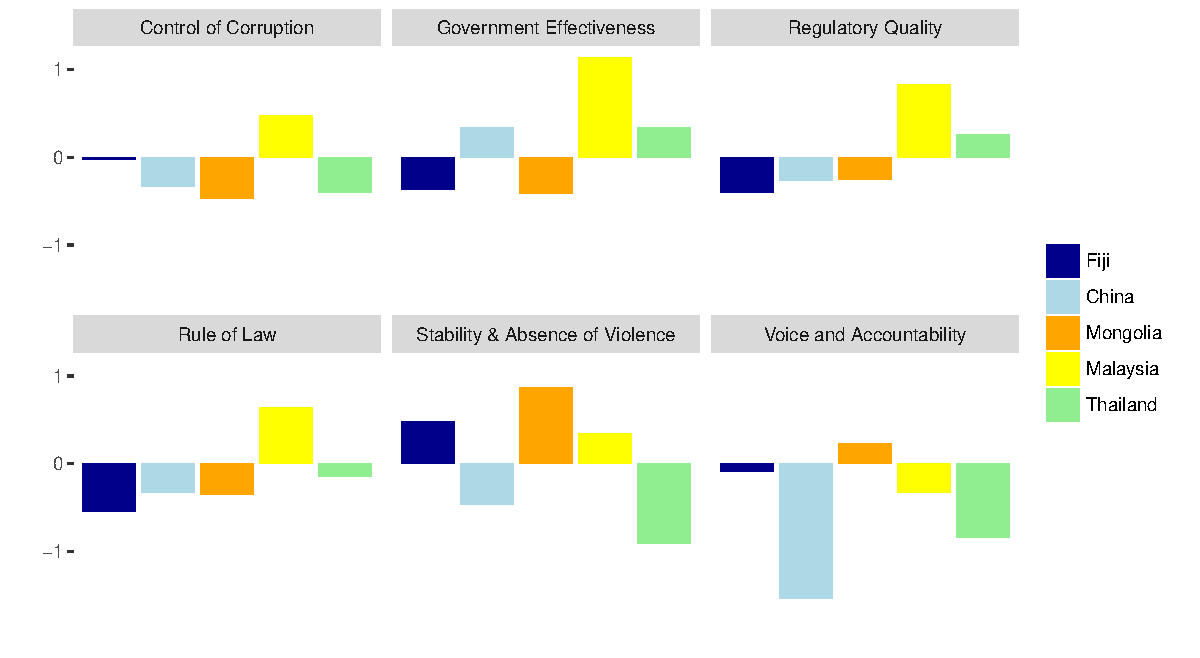
\includegraphics[width=\maxwidth]{figure/WGIindicators-1} 

}



    \vspace*{-0.6cm} 
    \hspace*{0.3cm} \raggedright\footnotesize{\href{http://data.worldbank.org/data-catalog/worldwide-governance-indicators}{Source: Worldwide Governance Indicators}}
  \end{minipage}
  \begin{minipage}[c]{0.48\textwidth} % Trade Policy table
    \vspace*{0.4cm}
  %\begin{flushleft}
    {\color{blue!50!black} \textbf{Trade Policy}}
  %\end{flushleft} 
  %\vspace*{0.2cm}
    \\[20pt]
    \centering
    \resizebox{\textwidth}{!}{%
% latex table generated in R 3.2.2 by xtable 1.7-4 package
% Tue May 31 11:05:34 2016
{\Large
\begin{tabular}{lrrr}
  & 2010 & 2013 &  \\ 
  \hline
Applied Tariff (Incl. Prefers. and Trade-Weighted) & 13.9 & 12.8 &  \\ 
  Binding (\%) & 15.7 & 15.3 &  \\ 
  Dispersion (Standard Deviation) & 9.3 & 9.7 &  \\ 
  Import duties collected (\%, 2011-2013) \large{[1]} & --- & 8.9 &  \\ 
  MFN Tariff (Agriculture) & 17.3 & 16.9 &  \\ 
  MFN Tariff (Non-Agriculture) & 13.7 & 12.9 &  \\ 
  MFN Tariff (Simple Average) & 14.4 & 13.6 &  \\ 
  Services sectors with GATS commitments \large{[1]} & --- & 9.0 &  \\ 
  \end{tabular}
}

    }
    \\[20pt]
    %\hspace*{0.5cm} 
    \raggedright{\footnotesize{\href{http://wits.worldbank.org}{Sources: WITS}{, }\href{http://stat.wto.org/CountryProfile/WSDBCountryPFHome.aspx?Language=E}{[1] WTO Trade Profiles}}}
  \end{minipage}
\end{minipage}

\vspace{+8ex}
%\hspace*{0.2cm}\subsection*{\color{white!50!black}Private Sector's Views}
\hspace*{0.1cm} \raggedright{\color{white!50!black}\Large Private Sector View}

\vspace*{-0.2cm}
{\color{white!30!black}\noindent\makebox[\linewidth]{\rule{18cm}{0.2pt}}} % horiz line

\begin{minipage}[b]{0.99\textwidth}
\vspace*{+0.6cm}
  \begin{minipage}[c]{0.02\textwidth}
  \hspace*{+0.1cm}
  \end{minipage}
  \begin{minipage}[c]{0.97\textwidth} 
    \begin{flushleft}  
      {\color{blue!50!black} \textbf{Enterprise Survey 2013}}
    \end{flushleft}  
    \vspace*{-0.4cm}
    \centering
    \resizebox{\textwidth}{!}{%
% latex table generated in R 3.2.2 by xtable 1.7-4 package
% Tue May 31 11:05:34 2016
{\Large
\begin{tabular}{lrrrl}
  & South Asia & Bangladesh & All Countries &  \\ 
  \hline
Number of electrical outages in a typical month & 25.40 & 64.50 & 6.30 &  \\ 
  Percent of firms with a bank loan/line of credit & 27.00 & 34.10 & 35.20 &  \\ 
  Proportion of investments financed by banks (\%) & 14.40 & 12.40 & 14.60 &  \\ 
  Proportion of investments financed internally (\%) & 73.90 & 74.50 & 71.20 &  \\ 
  Senior management time spent dealing with the requirements of government regulation (\%) & 7.20 & 3.30 & 10.00 &  \\ 
  \end{tabular}
}

    }
    \\[8pt]
    %\hspace*{0.3cm} 
    \raggedright{\footnotesize{\href{https://www.enterprisesurveys.org/data}{Source: Enterprise Survey 2013}}}
  \end{minipage} 

  \begin{minipage}[b]{0.99\textwidth} 
    \vspace{+4ex}
    \begin{minipage}[c]{0.49\textwidth} % top 5 constraints ES
      \center{\color{blue!50!black} \textbf{Top 5 constraints according to ES 2013 \\ \footnotesize(\% respondants)}}


{\centering 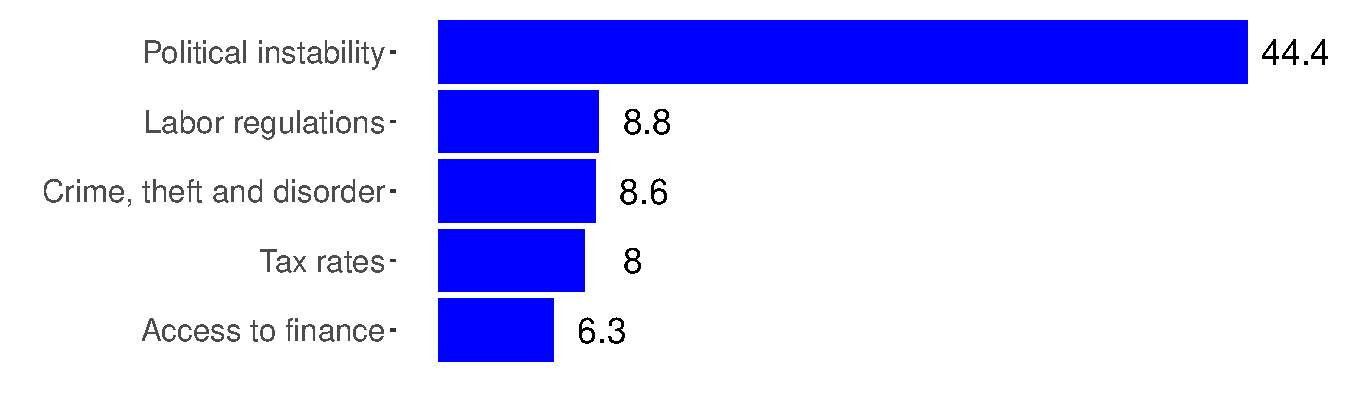
\includegraphics[width=\maxwidth]{figure/top5constraintsES-1} 

}



      %\vspace*{-0.7cm}
      \hspace*{0.3cm} \raggedright\footnotesize{\href{https://www.enterprisesurveys.org/data}{Source: Enterprise Survey 2013}}
    \end{minipage}
    \begin{minipage}[c]{0.49\textwidth} % top 5 constraints WEF
      \center{\color{blue!50!black} \textbf{Top 5 constraints according to WEF 2015 survey \\ \footnotesize(\% respondants among 88 executives)}}


{\centering 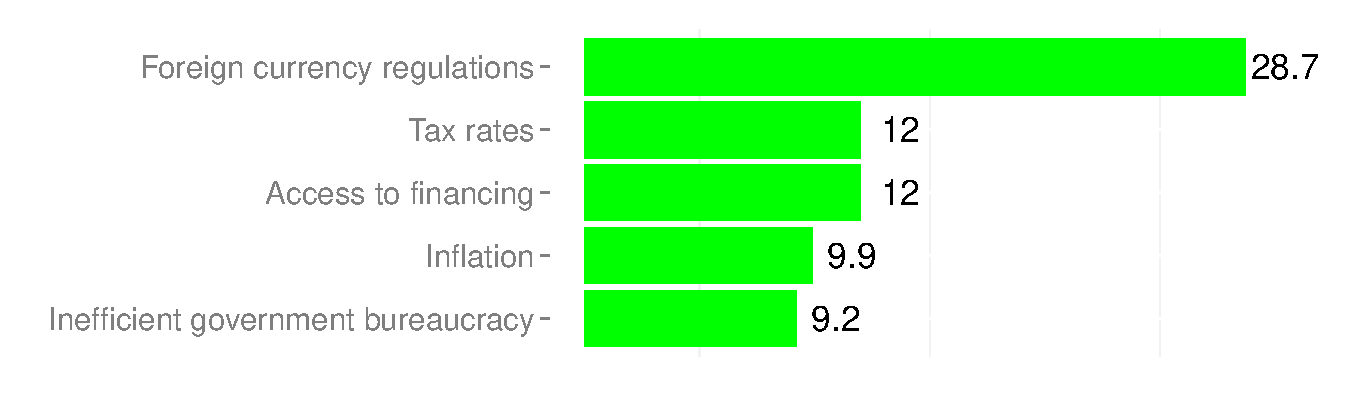
\includegraphics[width=\maxwidth]{figure/top5constraintsWEF-1} 

}



    %\vspace*{-0.7cm}
    \hspace*{0.3cm} \raggedright\footnotesize{\href{http://www.weforum.org/reports/global-competitiveness-report-2015-2016}{Source: WEF Global Competitiveness Report 2015}}
    \end{minipage}
  \end{minipage}
\end{minipage}

% \vspace{+8ex}
% {\color{blue!50!white}\noindent\makebox[\linewidth]{\rule{18cm}{0.3pt}}} % horiz line

% \vspace{+2ex}
% \begin{minipage}[c]{0.33\textwidth}
%   \hspace*{+0.3cm} \includegraphics[width=4cm,left]{/Users/asanchez3/shinyTCMN/www/wb_logo.jpg}
%   %\hspace*{+0.3cm} \includegraphics[width=4cm,left]{/Users/asanchez3/shinyTCMN/www/wb_logo.png}
% \end{minipage}
% \begin{minipage}[c]{0.65\textwidth}
%   \vspace*{-0.4cm}
%   \raggedleft{\color{white!40!black} \footnotesize TRADE AND COMPETITIVENESS MONITORING NOTE - UPDATED} 
%   %month year}
% \end{minipage}

%%%%%%%%%%%%%%%%%%%%%%%%%%%%%%%%%%%
%%%%%% Operations section %%%%%%%%%
%%%%%%%%%%%%%%%%%%%%%%%%%%%%%%%%%%%
\newpage
%%%%%%%%%%%%%%%% PAGE 3 %%%%%%%%%%%%%%%%%%%

%World Bank logo and TCMN branding
\begin{figure}
  \vspace{-3ex} % move up this figure
  \hspace{-7ex} % move left this figure
  \includegraphics[width=5cm]{/Users/asanchez3/shinyTCMN/www/wb_logo_background.png}
\end{figure}
\begin{figure}
  \begin{minipage}[t]{0.99\textwidth} % top section
      \vspace{-30ex}
      \hspace{-2ex}
      \raggedright{\includegraphics[width=5.5cm,right]{/Users/asanchez3/shinyTCMN/www/TC_snapshots_operations.png}}
  \end{minipage}
\end{figure}
%
%%%% Macro Indicators
\begin{minipage}[t]{0.99\textwidth} % top section
  \vspace{-1.5cm}
  \begin{minipage}[c]{0.36\textwidth} 
    \begin{minipage}[c]{0.28\textwidth} % flag
      \includegraphics[width=1.2cm,height=1.2cm]{/Users/asanchez3/shinyTCMN/www/BD.png}
    \end{minipage}
    \begin{minipage}[c]{0.70\textwidth} % Country name
      \section*{\color{blue!40!black}Bangladesh}
    \end{minipage}
  \end{minipage}
  \begin{minipage}[c]{0.63\textwidth}
  %  \begin{flushleft}  
  %    \center{\color{blue!20!black} \textbf{\Large T\&C Product Line Operations Board Approved On or After FY14}}
  %  \end{flushleft} 
  \end{minipage}  
\end{minipage} % end top section

%\begin{minipage}[b]{0.99\textwidth} % main body
  \raggedright{\color{white!30!blue} \textbf{\Large SCD/CPF}}
    \begin{minipage}[c]{0.99\textwidth}  
      \vspace*{0.2cm}
      \raggedright{\color{white!30!blue} \textbf{\large Most Recent}}
      \vspace*{0.3cm}
      
% latex table generated in R 3.2.2 by xtable 1.7-4 package
% Tue May 31 11:05:34 2016
\scalebox{0.85}{
\begin{tabular}{>{\raggedright}p{5in}ll}
 Product & Document Date &  \\ 
  \hline
Bangladesh - More and better jobs to accelerate shared growth and end extreme poverty & 2015-11-01 &  \\ 
  Bangladesh - Completion and learning review for the period FY2011-15 & 2016-04-05 &  \\ 
  \end{tabular}
}

      \vspace*{0.5cm}
    \end{minipage}
    
    \begin{minipage}[c]{0.99\textwidth} % imports/exports
      \vspace*{0.2cm}
      \raggedright{\color{white!30!blue} \textbf{\large Planned}}
      \vspace*{0.3cm}
      
% latex table generated in R 3.2.2 by xtable 1.7-4 package
% Tue May 31 11:05:34 2016
\scalebox{0.85}{
\begin{tabular}{>{\raggedright}p{5in}lll}
 Product & Concept Review Date & Board Date &  \\ 
  \hline
None &  &  &  \\ 
  \end{tabular}
}

      \vspace*{0.5cm}
    \end{minipage}
%\end{minipage}
  
\vspace*{0.5cm}
\raggedright{\color{white!30!blue} \textbf{\Large WB Lending Pipeline}}
\begin{minipage}[b]{0.99\textwidth} % overview tables
  \begin{minipage}[c]{0.99\textwidth}  
    \vspace*{0.5cm}
% latex table generated in R 3.2.2 by xtable 1.7-4 package
% Tue May 31 11:05:34 2016
{\footnotesize
\scalebox{0.85}{
\begin{tabular}{l>{\raggedright}p{1in}>{\raggedright}p{1in}>{\raggedright}p{0.5in}>{\raggedright}p{0.5in}>{\raggedright}p{0.5in}>{\raggedright}p{0.6in}>{\raggedright}p{0.5in}>{\raggedright}p{0.5in}>{\raggedleft}p{0.5in}>{\raggedleft}p{0.5in}l}
 Project ID & Project Name & Team Leader & Approval Date & Lending Inst. Type & Begin Appraisal & Commitment (US\$M) & Latest Sort Overall Risk Rating & FY Expenses (US\$K) & Cum Expenses (US\$K) & FY Prob &  \\ 
  \hline
P156113 & Developing High Potential Sectors & Bharatha Manju S. Haththotuwa & 2017-07-13 & IPF & 2017-04-17 & --- & --- & 0 & 0 & C &  \\ 
  \end{tabular}
}
}

    \vspace*{0.5cm}
  \end{minipage}
    
  \raggedright{\color{white!30!blue} \textbf{\Large WB Portfolio}}
  \begin{minipage}[c]{0.99\textwidth} % imports/exports
    \vspace*{0.2cm}
    \raggedright{\color{white!30!blue} \textbf{\large Active}}
    \vspace*{0.3cm}
      
% latex table generated in R 3.2.2 by xtable 1.7-4 package
% Tue May 31 11:05:35 2016
{\scriptsize
\scalebox{0.85}{
\begin{tabular}{l>{\raggedright}p{1in}>{\raggedright}p{1in}>{\raggedright}p{0.5in}>{\raggedright}p{0.5in}>{\raggedright}p{0.5in}>{\raggedleft}p{0.5in}>{\raggedleft}p{0.5in}>{\raggedright}p{0.4in}>{\raggedright}p{0.4in}>{\raggedright}p{0.4in}>{\raggedleft}p{0.4in}l}
 Project ID & Project Name & Team Leader & Approval Date & Lending Inst. Type & Closing Date & Commitment (US\$M) & Undisbursed Balance (US\$M) & Project Rating DO & Project Rating IP & Overall Risk & Months in Problem Status &  \\ 
  \hline
P156242 & PSDSP Additional Financing & Michael Olavi Engman & 2016-04-05 & IPF & --- & 130 &  --- & --- & --- & M & --- &  \\ 
  P120843 & BD: Private Sector Development Support & Michael Olavi Engman & 2011-03-01 & IPF & 2021-02-28 & 120 & 133 & S & S & S &  0 &  \\ 
  P117542 & BD: Invstmnt Prom \& Financing Facility & A.K.M. Abdullah & 2010-05-04 & IPF & --- & 257 &  --- & --- & --- & --- & --- &  \\ 
  \end{tabular}
}
}

    \vspace*{0.5cm}
  \end{minipage}
     
  \begin{minipage}[c]{0.99\textwidth} % imports/exports 
    \raggedright{\color{white!30!blue} \textbf{\large Closed}}
    \vspace*{0.5cm}
      
% latex table generated in R 3.2.2 by xtable 1.7-4 package
% Tue May 31 11:05:35 2016
{\footnotesize
\scalebox{0.85}{
\begin{tabular}{l>{\raggedright}p{1.5in}>{\raggedright}p{1in}>{\raggedright}p{0.5in}>{\raggedright}p{0.5in}>{\raggedright}p{0.5in}>{\raggedleft}p{0.6in}>{\raggedright}p{0.5in}>{\raggedright}p{0.5in}>{\raggedright}p{0.5in}l}
 Project ID & Project Name & Team Leader & Approval Date & Lending Inst. Type & Closing Date & Commitment (US\$M) & Project Rating DO & Project Rating IP & IEG Outcome Rating &  \\ 
  \hline
None &  &  &  &  &  &  &  &  &  &  \\ 
  \end{tabular}
}
}

    \vspace*{0.5cm}
  \end{minipage}
     
\end{minipage}
 
 \newpage
%%%%%%%%%%%%%%%% PAGE 2 %%%%%%%%%%%%%%%%%%%
\begin{minipage}[t]{0.99\textwidth}
  \raggedright{\color{white!30!blue} \textbf{\Large WB ASA}}

  \begin{minipage}[b]{0.99\textwidth}
    \vspace*{0.2cm}
    \raggedright{\color{white!30!blue} \textbf{\large Active}}
    \vspace*{0.3cm}
  
% latex table generated in R 3.2.2 by xtable 1.7-4 package
% Tue May 31 11:05:35 2016
{\scriptsize
\scalebox{0.85}{
\begin{tabular}{l>{\raggedright}p{1in}>{\raggedright}p{1in}>{\raggedright}p{0.6in}>{\raggedright}p{0.6in}>{\raggedright}p{0.4in}>{\raggedright}p{0.4in}>{\raggedleft}p{0.6in}>{\raggedleft}p{0.6in}>{\raggedleft}p{0.6in}>{\raggedleft}p{0.6in}l}
 Task ID & Task Name & Team Leader & Concept Approval Date & Output Approval Date & Product Line & RAS (Y/N) & Current Expenditure BB (US\$K) & Current Expenditure Total (US\$K) & Lifetime Expenditure BB (US\$K) & Lifetime Expenditure Total (US\$K) &  \\ 
  \hline
P156153 & Solar Irrigation with Electric Vehicle & Naoto Kanehira & 2015-12-04 & 2016-11-11 & TA & N & --- &   0 & --- &     0 &  \\ 
  P126702 & BD: PSDSP - Bank Exec Advisory Services & Bharatha Manju S. Haththotuwa & 2011-07-18 & 2016-06-29 & TA & N &  0 & 392 & 32 & 1,833 &  \\ 
  \end{tabular}
}
}

     \vspace*{0.2cm}
  \end{minipage}

  \begin{minipage}[b]{0.99\textwidth}
    \vspace*{0.2cm}
    \raggedright{\color{white!30!blue} \textbf{\large Closed}}
    \vspace*{0.3cm}
       
% latex table generated in R 3.2.2 by xtable 1.7-4 package
% Tue May 31 11:05:35 2016
{\scriptsize
\scalebox{0.85}{
\begin{tabular}{l>{\raggedright}p{1in}>{\raggedright}p{1in}>{\raggedright}p{0.6in}>{\raggedright}p{0.6in}>{\raggedright}p{0.4in}>{\raggedright}p{0.4in}>{\raggedleft}p{0.6in}>{\raggedleft}p{0.6in}>{\raggedleft}p{0.6in}>{\raggedleft}p{0.6in}l}
 Task ID & Task Name & Team Leader & Concept Approval Date & Output Approval Date & Product Line & RAS (Y/N) & Current Expenditure BB (US\$K) & Current Expenditure Total (US\$K) & Lifetime Expenditure BB (US\$K) & Lifetime Expenditure Total (US\$K) &  \\ 
  \hline
P149208 & IC-E-SCIENCE ED & Dilip Parajuli & --- & 2014-11-04 & KP & N & --- & 0 & 103 & 103 &  \\ 
  P147850 & 2ND JOBS AND COMPETITIVENESS & Vincent Palmade & --- & 2014-06-21 & TA & N & --- & 0 & 263 & 263 &  \\ 
  P123808 & BD: Diagnostic Trade Integration Study & Sanjay Kathuria & 2011-12-20 & 2014-04-12 & EW & N & --- & 0 & 272 & 658 &  \\ 
  P144654 & JOBS AND COMPETITIVENESS & Vincent Palmade & --- & 2013-06-25 & TA & N & --- & 0 & 124 & 124 &  \\ 
  P131789 & BD: JIT Note on IN/BD Trade & Sanjay Kathuria & --- & 2012-06-28 & TA & N & --- & 0 &  --- &   0 &  \\ 
  P117521 & BD: Trade Growth \& Diversification & Md. Abul Basher & --- & 2011-06-30 & EW & N & --- & 0 & 135 & 135 &  \\ 
  P103717 & Export Development and Diversification & Salomon Samen & --- & 2007-06-15 & TE & N & --- & 0 & 175 & 175 &  \\ 
  P103493 & Bangladesh Trade Growth and Poverty E-Le & Salomon Samen & --- & 2007-04-27 & TE & N & --- & 0 &  47 &  47 &  \\ 
  P103728 & Bangladesh WITS (World Int. Trade Sol.) & Salomon Samen & --- & 2007-03-08 & TE & N & --- & 0 &   2 &   5 &  \\ 
  P099476 & Bangladesh: World Integrated Trade Solut & Salomon Samen & --- & 2006-04-25 & TE & N & --- & 0 &   8 &   8 &  \\ 
  P098409 & Bangladesh: Services Trade Negotiations & Salomon Samen & --- & 2006-04-18 & TE & N & --- & 0 &  94 &  96 &  \\ 
  P077440 & Post MFA Strategic Options for RMG & Zaidi Sattar & --- & 2005-10-09 & EW & N & --- & 0 & 124 & 124 &  \\ 
  \end{tabular}
}
}

    \vspace*{0.5cm}
  \end{minipage}

  \raggedright{\color{white!30!blue} \textbf{\Large IFC ASA}}
  \begin{minipage}[b]{0.99\textwidth}
    \vspace*{0.2cm}
    \raggedright{\color{white!30!blue} \textbf{\large Active}}
    \vspace*{0.3cm}
  
% latex table generated in R 3.2.2 by xtable 1.7-4 package
% Tue May 31 11:05:35 2016
{\scriptsize
\scalebox{0.85}{
\begin{tabular}{l>{\raggedright}p{1.6in}>{\raggedright}p{1.5in}>{\raggedright}p{0.7in}>{\raggedright}p{0.7in}>{\raggedleft}p{0.7in}>{\raggedleft}p{0.7in}>{\raggedleft}p{0.7in}l}
 Project ID & Project Name & Team Leader & IP Approval Date & Expected End Date & Approval Value (in US\$K) & Total Expenditures (in US\$K) & Current FY Expenditure (in US\$K) &  \\ 
  \hline
584287 & Bangladesh IC for Industry- Agribusiness & Muhtaseb, Sherif & 2013-03-11 & 2015-12-31 & 2,456 & 2,470 & 425 &  \\ 
  585127 & Low-Carbon Industry Initiative in Bangladesh & Kechichian, Etienne Raffi & 2012-07-03 & 2013-12-26 &   860 &   882 &   1 &  \\ 
  584327 & Regulatory Modernization for supporting the creation of a Digital Bangladesh  & Ali, Miah Rahmat & 2011-06-29 & 2015-12-31 & 7,349 & 6,794 & 343 &  \\ 
  584527 & Business Taxation Streamlining Program & Babi, Nusrat Nahid & 2011-06-29 & 2015-12-31 & 4,100 & 3,979 & 276 &  \\ 
  \end{tabular}
}
}

    \vspace*{0.2cm}
  \end{minipage}

  \raggedright{\color{white!30!blue} \textbf{\large Pipeline}}
  \vspace*{0.3cm}
  
% latex table generated in R 3.2.2 by xtable 1.7-4 package
% Tue May 31 11:05:35 2016
{\scriptsize
\scalebox{0.85}{
\begin{tabular}{l>{\raggedright}p{1.6in}>{\raggedright}p{1.5in}>{\raggedright}p{0.7in}>{\raggedright}p{0.7in}>{\raggedleft}p{0.7in}>{\raggedleft}p{0.7in}>{\raggedleft}p{0.7in}l}
 Project ID & Project Name & Team Leader & IP Approval Date & Expected End Date & Approval Value (in US\$K) & Total Expenditures (in US\$K) & Current FY Expenditure (in US\$K) &  \\ 
  \hline
600422 & SME Ventures South Asia Phase 2 & Ni, Arsalan Alfred Ming Dode & --- & --- &      0 &   0 &   0 &  \\ 
  601054 & TAC Programmatic TA in Bangladesh & Reaz, M. Masrur & --- & 2020-12-31 & 20,200 & 115 & 115 &  \\ 
  \end{tabular}
}
}

  \vspace*{0.2cm}
\end{minipage}

\begin{minipage}[b]{0.99\textwidth}
  \raggedright{\color{white!30!blue} \textbf{\large Closed}}
  \vspace*{0.3cm}
  
% latex table generated in R 3.2.2 by xtable 1.7-4 package
% Tue May 31 11:05:35 2016
{\scriptsize
\scalebox{0.85}{
\begin{tabular}{l>{\raggedright}p{1.6in}>{\raggedright}p{1.5in}>{\raggedright}p{0.7in}>{\raggedright}p{0.7in}>{\raggedleft}p{0.7in}>{\raggedleft}p{0.7in}>{\raggedleft}p{0.7in}l}
 Project ID & Project Name & Team Leader & IP Approval Date & Expected End Date & Approval Value (in US\$K) & Total Expenditures (in US\$K) & Current FY Expenditure (in US\$K) &  \\ 
  \hline
571787 & GEM\_Promoting Gender Inclusion and Competitiveness in SEZs & Haider, Narissa & 2009-12-17 & 2012-12-31 &   595 &   578 & 0 &  \\ 
  570009 & BICF -Econ Zones & Muhtaseb, Sherif & 2009-10-01 & 2013-06-30 & 5,485 & 5,450 & 0 &  \\ 
  569887 & BICF Institutional Capacity Building & Watson, Laura Anne & 2009-09-29 & 2011-06-30 & 2,500 & 2,434 & 0 &  \\ 
  571047 & BICF-Regulatory Reform Phase 2 (FY 10-11) & Rahman, Mohammad Azad & 2009-09-29 & 2011-06-30 & 4,050 & 4,306 & 0 &  \\ 
  568007 & BICF Public Private Dialogue and Stakeholder Engagement Component & Watson, Laura Anne & 2009-05-29 & 2011-06-30 & 2,681 & 2,711 & 0 &  \\ 
  555689 & BICF Institutional Strengthening Component & Azhar, Shihab Ansari & 2008-02-19 & 2009-10-31 & 2,311 & 2,466 & 0 &  \\ 
  555688 & BICF-Regulatory Reform Component & Rahman, Aminur & 2007-12-04 & 2009-10-31 & 2,691 & 2,849 & 0 &  \\ 
  555686 & Bangladesh Investment Climate Fund - Economic Zones component & Rahman, Saika & 2007-11-20 & 2009-07-31 & 1,759 & 1,809 & 0 &  \\ 
  522487 & ICA Panel Survey & Wilson, Craig & 2006-02-24 & --- &     0 &     0 & 0 &  \\ 
  539143 & PILOTNG RFRM THROUGH DEVT \& MGMT OF ECONOMIC ZONES-BAN & Shah, Fatima Zehra & 2006-02-22 & --- &     0 &     0 & 0 &  \\ 
  538903 & FIAS Embedding Regulatory Reform in Bangladesh & Wilson, Craig & 2006-02-21 & --- &     0 &     0 & 0 &  \\ 
  541063 & PSD Reform Process Facilitation and Management & Crittle, Frederick J. & 2006-02-21 & --- &     0 &     0 & 0 &  \\ 
  541083 & Institutionalizing the PSD Regulatory Reform Process & Wilson, Craig & 2006-02-21 & --- &     0 &     0 & 0 &  \\ 
  541084 & Assessing and Addressing Stakehholder Interests in PSD Reform & Crittle, Frederick J. & 2006-02-21 & 2006-11-30 &   126 &    88 & 0 &  \\ 
  538472 & Facilitation of PSD Vision and Monitoring and Evaluation System & Rahman, Aminur & 2006-02-08 & --- &     0 &     0 & 0 &  \\ 
  522103 & DCCI Diagonostics & Molla, Md. Akhtar Uddin & 2005-12-30 & --- &     0 &     0 & 0 &  \\ 
  541363 & FIAS RIA BANGLADESH: A---LYSIS, SOLUTION DESIGN AND PILOTS & Ladegaard, Peter Farup & 2005-11-13 & 2007-06-30 &   142 &   106 & 0 &  \\ 
  533046 & Rountables on Free Zones and Regulatory Reform in Bangladesh & Gauthier, Jean Paul & 2005-08-15 & --- &     0 &     0 & 0 &  \\ 
  523296 & Investment Incentives Review & Crittle, Frederick J. & 2005-08-11 & --- &     0 &     0 & 0 &  \\ 
  532117 & High-Level Roundtable on Regulatory Reform & Crittle, Frederick J. & 2005-08-11 & --- &     0 &     0 & 0 &  \\ 
  523335 & Improving Systems and Automation at the Registrar of Joint Stock Companies, Bangladesh & Qayyum, Sayef Tanzeem & 2005-07-10 & 2008-12-31 & 1,082 & 1,179 & 0 &  \\ 
  532404 & Non-Tariff Barrier Advocacy and Bangladesh-North East India Secretariat & Haider, Narissa & 2005-07-10 & --- &     0 &     0 & 0 &  \\ 
  532908 & General System of Preference and SAARC Cumlation Research and Advocacy Project & Werner, Wendy Jo & 2005-07-10 & 2009-06-30 &     0 &    52 & 0 &  \\ 
  535883 & Trade Needs Assessement - Bangladesh & Haider, Narissa & 2005-07-10 & --- &     0 &     0 & 0 &  \\ 
  536827 & Advocacy Program for the Apparel Sector of Bangladesh & Werner, Wendy Jo & 2005-07-10 & --- &     0 &     0 & 0 &  \\ 
  \end{tabular}
}
}

  \vspace*{0.2cm}
\end{minipage}
%%%%%%%%%%%%%%%% END OF DOCUMENT %%%%%%%%%%%%%%%%%%%
\end{document}
